\documentclass[specialist,
               substylefile = spbu.rtx,
               subf,href,colorlinks=true, 12pt]{disser}

\usepackage[a4paper,
            mag=1000, includefoot,
            left=3cm, right=1.5cm, top=2cm, bottom=2cm, headsep=1cm, footskip=1cm]{geometry}
\usepackage[T2A]{fontenc}
%\usepackage{ucs}
\usepackage[cp1251]{inputenc}
\usepackage[english, russian]{babel}
\usepackage{indentfirst}
\usepackage{amsmath}
\usepackage{array}
\usepackage{graphicx}
\usepackage{verbatim}
\usepackage{hyperref}
\usepackage{color}
\usepackage{hyperref}
\usepackage{breakurl} 
\usepackage{url}
\usepackage{amssymb}
\usepackage{mathtools}
%\usepackage{subfigure}
\usepackage{xcolor}
\usepackage{tipa}
\usepackage{upgreek}
\usepackage{listings}
\usepackage{longtable}
\usepackage{caption}
%\hypnenation{гамма--рас-пре-де-ле-ние}
\usepackage{textcomp}
\DeclareCaptionFont{white}{\color{white}} %делает текст заголовка белым
%код ниже нарисует серую рамочку вокруг заголовка кода
\DeclareCaptionFormat{listing}{\colorbox{gray}{\parbox{\textwidth}{#1#2#3}}}
\captionsetup[lstlisting]{format=listing,labelfont=white,textfont=white}
\usepackage{marvosym}
\usepackage{amsthm}
\newtheorem{mydef}{Определение}
\newtheorem{myth}{Теорема}
\newtheorem{mynote}{Замечание}
\newtheorem{mylemma}{Лемма}
\newtheorem{myexample}{Пример}
\newtheorem{mycon}{Предложение}
\DeclareMathOperator{\h}{h}
\DeclareMathOperator{\const}{const}
\DeclareMathOperator{\argmin}{argmin}
%\DeclareMathOperator{\max}{max}
\ifpdf\usepackage{epstopdf}\fi

%\bibliographystyle{gost2008}
% Точка с запятой в качестве разделителя между номерами цитирований
%\setcitestyle{semicolon}

% Использовать полужирное начертание для векторов
\let\vec=\mathbf

% Включать подсекции в оглавление
\setcounter{tocdepth}{2}

\graphicspath{{fig/}}

%----------------------------------------------------------------
\begin{document}

% Название организации
\institution{%
    Санкт-Петербургский государственный университет \\
    Математико--механический факультет \\
    Кафедра статистического моделирования
}

% Имя лица, допускающего к защите (зав. кафедрой)
%\apname{д.\,ф.-м.\,н., профессор С.\,М.~Ермаков}

\title{Конспект}

% Тема
\topic{\normalfont\scshape%
     Построение минимальных идеальных хэш--функций с помощью случайных графов}

% Автор
\author{Алиева Наталия}


% Город и год
\city{Санкт-Петербург}
\date{\number\year}

\maketitle

\tableofcontents

\intro

Сегодня приходится работать с большими объемами данных, и с каждым днем их становится все больше. Вследствие этого  для экономии ресурсов требуется эффективно хранить имеющиеся данные. Кроме того, возникает необходимость быстрого доступа к каким--либо элементам наборов данных.

Стандартным решением для структуризации данных является \textbf{хэширование}. Каждому элементу присваивается некий индекс, а далее, когда нам необходимо получить доступ к какому-то элементу мы ищем его по списку индексов. Таким образом, перед нами встает задача индексации: построить некий ассоциативный словарь.

\subsubsection{О задачах и методах}

Если мощность множества ключей заранее неизвестна, применяется \textbf{стандартная процедура хэширования}: кроме основной памяти, выделяется резервная память. Тогда вернуть какой-то элемент множества можно в среднем за $\mathit{O}(1)$. Если же нам известна мощность множества ключей, можем также воспользоваться вышеописанным методом. Однако, имея такое ценное знание, как мощность исходного множества ключей, хочется получить какой-то более оптимальный способ хэширования.

Рассмотрим \textbf{частный случай}: пусть у нас есть конечный алфавит и конечное множество ключей, которые являются конечными строками. С одной стороны, можно было бы просто присвоить каждому элементу множества какой-то индекс и упорядочить, получив, таким образом, взаимно однозначное отображение. Действительно, при небольшой мощности нашего множества, такой способ прост в реализации и даст результат за время $\mathit{O}(n)$, где $n$ --- мощность множества строк. С другой стороны, с ростом $n$ время выполнения операции увеличивается линейно, и при достаточно больших $n$ операция становится трудозатратной.

Можно также воспользоваться описанным выше способом хэширования для множества ключей любой мощности. Тогда вернуть какой-то элемент множества можно в среднем за $\mathit{O}(1)$. А можно ли лучше?

\subsubsection{Постановка задачи}

Найти такую биективную хэширующую функцию, которая вычисляет значение в точке за $\mathit{O}(1)$, и, кроме того, придумать алгоритм, который будет строить такую функцию за время $\mathit{O}(n)$.
\\

\textbf{Минимальные идеальные хэширующие функции (minimal perfect hash functions)} --- один из инструментов, который помогает решить такую проблему. Такие функции широко применяются во многих сферах, например:

\begin{itemize}
\item естественные языки,
\item зарезервированные слова в языке программирования,
\item URLs,
\item Data Mining: нестандартные взаимосвязи между переменными в больших базах данных.
\end{itemize}

В этом конспекте будет рассматриваться задача построения минимальных идеальных хэш--функций с помощью случайных графов на примере одного из алгоритмов.

\newpage

\section{Вспомогательные определения. Случайные графы.}

\begin{mydef}
\textbf{Случайный граф} --- это общий термин для определения вероятностного распределения графов.
\end{mydef}

Случайные графы описываются \textbf{распределением вероятности} или \textbf{случайным процессов}, создающим эти графы.

Пусть множество вершин фиксировано, и над множеством подмножеств множества ребер задано некоторое распределение. Таким образом, имеется $n$ вершин и  $N$ ребер, при этом максимально возможное число ребер равняется $\binom{n}{2}$; добавляем последовательно и независимо ребра, соединяющие эти вершины, с некоторой вероятностью $p \in (0;1)$. Таким образом, получается граф $G(n,p)$: любое ребро появляется с вероятностью $p$.

Пусть также $0 \leq M \leq N$. Тогда вероятность появления графа $G(n,p)$ с $M$ ребрами:
%
\begin{equation}
p^M(1-p)^{N - M}.
\end{equation}
%

Самая распространенная модель случайного графа --- это \textbf{модель Эрдёша-Реньи}: в ней все $\binom{\binom{n}{2}}{n}$ графов на $V$ с $n$ вершинами равновероятны. Ее мы и будем рассматривать далее.


\newpage

\section{Построение минимальных идеальных хэш--функций}

\textbf{Минимальная идеальная хэш--функция} --- по сути своей является биективной хэш--функцией. 

Существует много способов построения таких функций, ниже приведены некоторые из них:

\begin{itemize}
\item[1.] Форма результирующей функции такова: $h(x) = (f(x) + d_{g(x)}) \mod n$, где $f$ и $g$ из семейства \textbf{универсального множества хэш--функций}, а $d$ --- множество значений перестановок, которые разрешают коллизии, производимые функцией $f$. Определив множество условий относительно $f$ и $g$ и показав, что эти условия выполняются, можно вычислить минимальную идеальную хэш--функцию $h$ за ожидаемое время $\mathit{O}(n)$
\item[2.] Алгоритм, основанный на построении \textbf{нециклического} графа. Выбираем случайным образом хэш--функции $h_1$ и $h_2$ из семейства универсальных хэш--функций пока граф $G$, построенный на их основе, не будет нециклическим. Далее на основе полученного графа $G$ строится минимальная идеальная хэш--функция с \textbf{сохранением порядка} (минимальная идеальная хэш--функция называется \textit{сохраняющей порядок}, если она сохраняет порядок ключей в исходном множестве и переносит его в результирующую хэш--таблицу).\label{alg2}
\end{itemize}

Здесь и далее представлена модификация метода построения минимальных идеальных хэш--функций \textbf{MOS (Mapping--Ordering--Searching)}, основанный на случайных графах (\textbf{пункт 2}).
Основная идея метода заключается в построении случайного графа и установления взаимно однозначного отображения между множеством его вершин и множеством ключей. В отличие от вышеописанного метода, построенный в нашем случае граф может быть, в каком--то смысле, произвольным, то есть содержать циклы, поэтому для оптимальной работы алгоритма будем работать не с целым графом сразу, а с его частями: \textbf{циклической} и \textbf{нециклической} частью. В этом и состоит \textbf{особенность реализации алгоритма}.

Метод состоит из следующих этапов:

\begin{itemize}
\item \textbf{Mapping}: формирование случайного графа.
\item \textbf{Ordering}: скорее partition --- разбиение множества вершин графа на, так называемые, циклическую и не циклическую часть.
\item \textbf{Searching}: формирование отображения между множеством ключей множеством вершин графа.
\end{itemize}

Для начала введем обозначения. Пусть $S$ --- множество из $n$ строк (ключей) конечной длины над конечным алфавитом $\Sigma$.
Определим также $h: S \longrightarrow M$ ---  некая хэш--функция. Для данного ключа $x \in S$ хэш--функция $h$ вычисляет целое значение в промежутке $[0;m-1]$ для обозначения уникального адреса  $x$ в хэш--таблице. В этом конспекте пойдет речь только о статических множествах ключей (заранее известным набором ключей, который не меняется со временем).

Для заданного множества ключей $S$ будем говорить, что $h: S \longrightarrow M$ --- \textbf{идеальная хэш--функция} для $S$, если $h$ является \textbf{инъекцией} на $S$ (нет ни одной \textbf{коллизии} среди ключей в $S$). Если, кроме того, $m = n$ (то есть $h$ является биекцией), тогда $h$ называют \textbf{минимальной идеальной хэш--функцией}. Покажем теперь, как строится такая функция.

Рассмотрим 2 вспомогательные функции (о том, как выбрать $h_1$ и $h_2$, мы поговорим позже) $h_1, h_2 : S \longrightarrow V$, где $V = [0; t-1]$ для некоторого выбранного подходящего целого $t = cn$, где $n = |S|$. Построим граф $G = G(h_1, h_2)$ на $V$ такой, что: $E(G) = \{\{h_1(x),h_2(x)\}: x \in S\}$. Для каждого ключа в множестве ключей $S$ существует ребро в графе $G$.

Здесь и далее будем рассматривать максимальный подграф графа $G$ сo степенью не меньше 2. Такой подграф будем называть \textbf{критическим подграфом} графа $G$ и обозначим его как $G_{crit}$. Вершины и ребра такого подграфа также называются \textbf{критическими}: $V_{crit} = V(G_{crit})$, $E_{crit} = E(G_{crit})$. Кроме того, дополнения к множеству критических вершин и ребер будем называть \textbf{некритическими вершинами и ребрами}: $V_{ncrit} = V \setminus V_{crit}$, $E_{ncrit} = E \setminus E_{crit}$. Введем также $V_{scrit} \subseteq V_{crit}$ --- множество всех критических вершин, у которых есть хотя бы одна некритическая вершина в качестве соседа. Таким образом, \textbf{некритический подграф} графа $G$ построен следующим образом: $G_{ncrit} = (V_{ncrit} \cup V_{scrit}, E_{ncrit})$. Некритический подграф относится к нециклической части графа. В итоге получаем $G = G_{crit} \cup G_{ncrit}$.

Построим теперь подходящую раскраску $g : V \longrightarrow \mathbb{Z}$ для вершин графа $G$: для каждой $v \in G$ выбираем такую $g(v)$, что $h(x) = g(h_1(x)) + g(h_2(x))$ (при $x \in S$), где $h$ --- минимальная идеальная функция хэширования для $S$.

В итоге рассматриваемый алгоритм действует следующим образом: на вход получает множество ключей $S$, а в качестве результата возвращает маркировку $g$. На самом деле такая раскраска $g$ может быть найдена при условии: $|E(G_{crit})| \leq \frac{1}{2}|E(G)|$. Это будет освещено в разделе ~\ref{sec:mapan}.

\begin{figure}[h]
\begin{center}
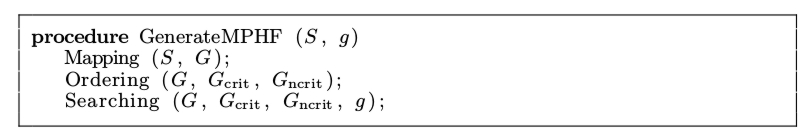
\includegraphics[scale=0.5]{imgs/proc.jpg}
\caption{Основные шаги алгоритма по построению минимальных идеальных хэш--функций}
\end{center}
\end{figure}
Представим далее каждый шаг более подробно.

\subsection{Mapping step}

Шаг $Mapping (S, G)$ получает на вход множество ключей $S$ и строит случайный граф $G = G(h_1, h_2)$  генерированием 2--х вспомогательных функций $h_1, h_2 : U \longrightarrow [0;t - 1]$ (как именно строится случайный граф $G$, мы рассматривать не будем). Это независимые функции, которые переводят множество слов $U$ в множество $[0; t - 1]$.

Рассмотрим вид функций $h_1, h_2$. Каждая из них получается следующим образом:
%
\begin{equation}\label{eq:1}
h_j(x) = \Big ( \sum \limits_{i = 1}^{|x|}T_j(i,x[i])\Big)\mod t,
\end{equation}
%
где $T_j$ --- функция, которая возвращает значение в соответветствующей хэш--таблице для конкретного символа и конкретной позиции этого символа слова $x$, при этом $|x| \leq L$ (таблица $T_j$ выглядит как игральное поле для морского боя: по вертикали идут цифры, то есть номера позиций в слове, они могут принимать значения от 1 до $L$, а по горизонтали выстроены все символы алфавита $\Sigma$).

Таким образом, для построения функций $h_1$ и $h_2$ нам необходимо сначала выбрать таблицы $T_1$ и $T_2$, затем сгенерировать $h_1$ и $h_2$ на основании ~\ref{eq:1}. Очевидно, что нельзя выбрать любые таблички $T_1$ и $T_2$ и сгенерировать произвольные $h_1$ и $h_2$. Давайте подумаем, какими свойствами должны обладать функции $h_1$ и $h_2$, вернемся для этого к нашему графу $G$.

Случайный граф $G = G(h_1, h_2)$ имеет набор вершин $V = [0;t - 1]$ и ребер $E = \{\{h_1(x),h_2(x)\}: x \in S\}$. Необходимо, чтобы граф $G$ был простым, то есть не имел ни петель ни кратных ребер.

Петли будут возникать при $h_1(x) = h_2(x)$. для некоторых $x \in S$. Чтобы этого не было, выбираем вспомогательные функции так, что: $h_2(x) = (2h_1(x) + 1)\mod t$. Если после этого все же встречаются петли, тогда выбираем $h_1$ и $h_2$ заново. Если также встречается кратное ребро, прерываем процедуру и генерируем вспомогательные функции заново.

\subsection{Анализ шага Mapping} \label{sec:mapan}

Рассмотрим случайный граф $G = (V,E)$, где $|V| = t$ и $|E| = n$. Положим $d = \frac{2n}{t}$ --- среднее всех степеней вершин графа $G$. Автори статьи приводят следующий факт: если $d > 1$ или, что эквивалентно, $c < 2$ (напомним, что $t = cn$), тогда \textbf{почти любой} граф $G$ содержит ``гигантскую'' компоненту, то есть большая часть вершин будет задействована в связной компоненте графа.

Вернемся к построению нашего графа $G$ на основе $h_1$ и $h_2$. Если $h_1$ и $h_2$ уже известны, то шаг $Mapping$ поддается теоретическому анализу. Авторы статьи представили свои результаты для критической компоненты подграфа. Таким образом, число вершин $G_{crit}$ равно (без док--ва):
%
\begin{equation}\label{eq1}
|V(G_{crit})| = (1+\mathit(o)(t))(1 - T)bt,
\end{equation}
%
почти наверное. Кроме того, число ребер в этом графе (без док--ва):
%
\begin{equation}\label{eq2}
|E(G_{crit})| = (1+\mathit{o}(1))\Big((1-T)b + b(d + T - 2)/2\Big)t,
\end{equation}
%
почти наверное. 
Временная сложность этого шага $\mathit{O}(n)$.

\newpage

\subsection{Ordering step}

Процедура упорядочивания $Ordering (G, G_{crit}, G_{ncrit})$ получает на вход граф $G$ и на выходе возвращает два подграфа: критический $G_{crit}$ и некритический $G_{ncrit}$ такие, что $G = G_{crit} \cup G_{ncrit}$. Чтобы достичь этого результата, будем итеративно удалять все вершины степени 1, пока таковых не останется. Рассмотрим действие этого шага алгоритма на примере.

\begin{myexample}
Рассмотрим граф с 9--ю вершинами и 8--ю ребрами, где степень вершины \textbf{d} для каждой вершины указана над соответствующей вершиной.

\begin{figure}[h]
\begin{center}
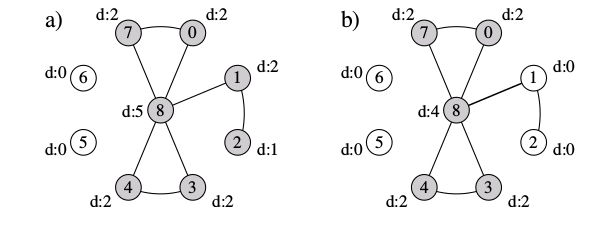
\includegraphics[scale=0.5]{imgs/ex2.jpg}\label{im:ex2}
\caption{Пример разбиения исходного графа на два подграфа: критический и некритический}
\end{center}
\end{figure}

Применяя шаг упорядочивания к графу на рисунке ~\ref{im:ex2}, в итоге оценили граф из 5--ти вершин. Получили, что все вершини степени 0 являются некритическими вершинами, а все остальные --- критическими. Чтобы определить вершины множества $V_{scrit}$, соберем все вершины $v \in V(G_{crit})$, у каждого из которых хотя бы одна вершина принадлежит списку смежных вершин для $v$ и множеству $V(G_ncrit)$, как вершина 8 на рисунке ~\ref{im:ex2}.
\end{myexample}

Отметим, что временная сложность этого шага $\mathit{O}(|V(G)|)$. Так как $|V(G)| = t = cn$, этап упорядочивания происходит за время $\mathit{O}(n)$.

\newpage

\subsection{Searching step}

На шаге $Searching (G, G_{crit}, G_{ncrit}, g)$ на вход подаются исходный граф $G$ и подграфы $G_{crit}, G_{ncrit}$, и процедура поиска ищет подходящее значение в массиве $g$ для каждой вершины $v \in V(G)$. Сначала на этом шаге обрабатываются вершины критического подграфа $G_{crit}$, а затем вершины некритического подграфа $G_{ncrit}$. Это необходимо, чтобы разрешить все переобозначения как можно раньше (такие переобозначения могут быть вследствие наличия циклов в подграфе).

\subsubsection{Присваивание значений для критических вершин}

Метки $g(v) (v \in V(G_{crit}))$ назначаются в порядке возрастания, следуя жадной стратегии, где критические вершины рассматриваются по одному, согласно поиску в ширину в подграфе $G_{crit}$. Если предлагаемое значение $x$ для $g(v)$ запрещено (такое присвоение $g(v) = x$ создаст 2 ребра с одинаковым весом), тогда увеличиваем $x$ на 1 и пробуем присвоить $g(v)$ $x+1$.

Пусть множество $A_E$ --- множество адресов, присвоенных ребрам в $E(G_{crit})$. Изначально $A_E = \emptyset$. Пусть $x$ --- кандидат для $g(v)$. Изначально $x = 0$. Считая, что подграф $G_{crit}$ имеет вид~\ref{im:ex2}, рассмотрим пошаговый пример присваивания значений вершинам в подграфе $G_{crit}$ на рисунке~\ref{im:ex3}.

Итак, у нас выбрана вершина $v$, необходимо присвоить предлагаемое значение $x$ в случае успеха, затем увеличит $x$ на 1 и так далее. Допустим, выбранная вершина -- \textbf{№8}, значит $g(8) = 0$, и $x$ становится 1. Теперь рассмотрим все вершины из списка смежности для вершины \textbf{№8}. Сначала рассмотрим вершину \textbf{№0}. В этом случае соберем в множество $Y$ те вершины, которые уже имеют присвоенное значение $x$ и которые смежные к \textbf{№0}, т.е. $Y = \{8\}$. Далее для всех $u \in Y$ проверяем условие: $g(u) + x \notin A_E$.

\begin{figure}[h]
\begin{center}
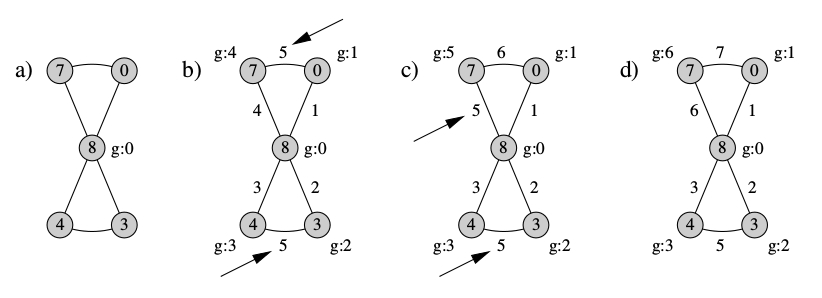
\includegraphics[scale=0.35]{imgs/ex3.jpg}\label{im:ex3}
\caption{Пример присваивания значений вершинам критического подграфа}
\end{center}
\end{figure}


Так как $g(8) + 1 = 1 \notin A_E$, значит 1 присваивается $g(0)$, $x$ становится 2, и пополняется множество $A_E$: $A_E = A_E \cup \{1\} = \{1\}$. Далее рассматриваем вершину \textbf{№3}, $g(3)$ присваивается 2,  и $A_E = A_E \cup \{2\} = \{1,2\}$. Затем достигается вершина \textbf{№4}, и $Y = \{3,8\}$. Так как $g(3) + 3 = 5 \notin A_E$ т $g(8) + 3 = 3 \notin A_E$, тогда $g(4)$ присваивается 3, а $A_E = A_E \cup \{3,5\} = \{1,2,3,5\}$. Наконец, достигли вершины \textbf{№7}, и $Y = \{0,8\}$. $g(0) + 4 = 5 \in A_E$, $x$ увеличивается на 1 ($x = 5$). $g(8) + 5 = 5 \in A_E$, тогда $x$ еще увеличивается на 1 ($x = 6$). Снова проверяем: $g(0) + 6 = 7 \notin A_E$ и $g(8) + 6 = 6 \notin A_E$, тогда $g(7)$ присваивается 6, кроме того, $A_E = A_E \cup \{6,7\} = \{1,2,3,5,6,7\}$. Этим завершается алгоритм, так как все вершины критического подграфа рассмотрены.

\subsubsection{Присваивание значений для некритических вершин}

В этом случае мы производим назначение значений к вершинам некритического подграфа из неиспользованных значений на предыдущем шаге. Поэтому начинаем поиск в глубину в $V_{scrit}$, так как метки $g$ на эти вершины уже расставлены и не могут меняться. Считая некритический подграф таким, как на рисунке~\ref{im:ex2} рассмотрим пошаговый пример присвоения значений.Выбираем вершину, с которой начнем (в данном случае снова \textbf{№8}) и идем последовательно.

\begin{figure}[h]
\begin{center}
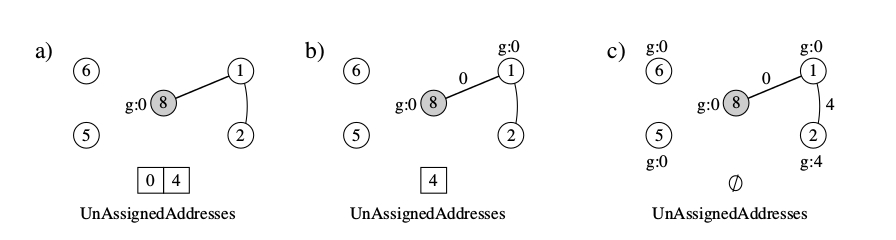
\includegraphics[scale=0.35]{imgs/ex4.jpg}\label{im:ex4}
\caption{Пример присваивания значений вершинам некритического подграфа}
\end{center}
\end{figure}

В предыдущем примере остались неиспользованными вершины $\{0,4\}$. Таким образом, берем 0 --- как первый неиспользованный адрес и вершину \textbf{№1} --- как вершину, смежную к \textbf{№8}. $0 - g(8) = 0$ (``адрес'' - ``значение в исходной вершине''), поэтому $g(1)$ присваивается 0. И единственная неохваченная вершина: $4 - g(1) = 4$, поэтому $g(2)$ присваиваем 4. Свободным вершинам присваивается 0. Процесс продолжается, пока список неотмеченных вершин не пуст.

\subsection{Анализ шага Searching}
Авторы статьи приводят доказательство следующих пунктов: 

\begin{itemize}
\item максимальное значение, присвоенное ребру $\leq n - 1$ (то есть мы действительно сгенерировали минимальную идеальную хэш--функцию),
\item задача определения раскраски $g$ может быть решена за ожидаемое время $\mathit{O}(n)$, если число ребер в $G_{crit}$ $\leq \frac{1}{2}|E(G)|$. 
\end{itemize}

Мы же рассмотрим в этом разделе только оценку временной сложности, опустив промежуточные теоретические результаты.

Мы заостряем внимание только на анализе распределения значений по критическим вершинам, так как аналогичная задача для некритических вершин решается за линейное время поиском в глубину.

Определим меры сложности. Пусть $I(v)$ --- сколько раз увеличивалось рассматриваемое значение $x$ для $g(v)$. Пусть также $N_{t}$ --- сколько всего раз рассматриваемое значение $x$ увеличивалось. Таким образом, получаем: $N_{t} = \sum \limits_{v \in V(G_{crit})} I(v)$.

Для простоты положим, что $G_{crit}$ связный. 

Авторы метода на основании теоретических и экспериментальных результатов в статье для дальнейшего вычисления временной сложности предполагают следующее: $N_{t} = |E(G_{crit})| - |V(G_{crit})| + 1$.

\subsubsection{Временная сложность}

Покажем, что временная сложность определения $g(v)$ для всех критических вершин $x \in V(G_{crit})$ равняется $\mathit{O}(|V(G_{crit})|) = \mathit{O}(n)$. Для каждой необозначенной вершины $v$ список смежности вершины $v$, $Adj(v)$, должен препятствовать формированию множества $Y$ смежных вершин, которым уже присвоили какое-то значение. Затем для каждой вершины из $Y$ мы проверяем, запрещено ли использовать $x$ (грубо говоря, проверяем приналежность суммы весов на вершинах множеству $A_E$, нам важно, чтобы для нового элемента сумма с другими смежными вершинами не была одинаковой). В итоге ребро, соединяющее $u$ и $v$ для всех $u \in Y$ связано в адресом, который соответствует сумме его конечных точек. Положим $d_{crit} = 2|E(G_{crit})|/|V(G_{crit})|$ среднее по всем степеням вершин подграфа $G_{crit}$. Заметим, что $|Y| \leq |Adj(v)|$ (для простоты будем предполагать, что $|Adj(v)| = \mathit{O}(d_{crit})$). Затем исходя из всего, указанного выше, временная сложность этой процедуры вычисляется следующим образом:
\begin{equation}
\begin{split}
\mathit{C}(|V(G_{crit})|) = \sum \limits_{v \in V(G_{crit})}\Big[ |Adj(v)| + (I(v) \times |Y|) + |Y|\Big] \leq \\
\sum \limits_{v \in V(G_{crit})} |Adj(v)|(2 + I(v)) = 4|E(G_{crit})| + \mathit{O}(N_{t}d_{crit}).
\end{split}
\end{equation}
Из предыдущего раздела(~\ref{secmax}) получается, что $d_{crit} = 2 \times 0.501n/0.401n \simeq 2.499$ (константа). Из этого следует, что $\mathit{O}(|E(G_{crit})|) = \mathit{O}(|V(G_{crit})|)$. Предполагая, что $N_{t} \leq N_{bedges}$, из теоремы~\ref{th1} получается: $N_{t} \leq |E(G_{crit})| - |V(G_{crit})| + 1 = \mathit{O}(|E(G_{crit})|)$. Таким образом, $\mathit{C}(|V(G_{crit})|) = \mathit{O}(|E(G_{crit})|) = \mathit{O}(|V(G_{crit})|)$. Так как $|V(G_{crit})| \leq |V(G)|$ и $|V(G)| = cn$, требуемое время для определения раскраски $g$ критических вершин $\mathit{O}(n)$.

\newpage

\conclusion

В этом разделе пойдет речь о плюсах и минусах рассмотренного алгоритма.
\\

\textbf{Преимущества:}
\begin{itemize}
\item Как уже было сказано ранее, алгоритм отличается тем, что при построении минимальной идеальной хэш--функции может обрабатывать не только нециклические графы, но и графы с циклической частью.
\item По сравнению с алгоритмом, описанном в пункте~\ref{alg2} (основан на построении нециклического графа), текущий строит граф с меньшим числом вершин.
\end{itemize}

\textbf{Недостатки:}
\begin{itemize}
\item В отличие от алгоритма, описанного в пункте~\ref{alg2} (основан на построении нециклического графа), текущий не сохраняет порядок ключей в исходном множестве при построении минимальной идеальной хэш--функции. Пример, когда нам это важно: поиск строки в базе по префиксу строки.
\item При анализе шага \textbf{Searching} не доказано теоретически допущение $N_{t} \leq N_{bedges}$, авторы алгоритма объясняют его лишь эмпирически.
\item Нет формального доказательства, что алгоритм работает всегда. Приведены хорошие результаты только на некоторых данных, о коих ничего неизвестно.
\end{itemize}


\end{document}
